\documentclass[letterpaper,12pt]{article}
\usepackage[utf8]{inputenc}
\usepackage[top=1.25in, bottom=1.25in, left=1in, right=1in]{geometry}
\usepackage{amsmath}
\usepackage{amsfonts}
\usepackage{enumitem}
\usepackage{graphicx}

\setenumerate{parsep=0em, listparindent=\parindent}

\DeclareMathOperator{\Tr}{Tr}
\DeclareMathOperator{\dom}{dom}
\DeclareMathOperator{\diag}{diag}
\DeclareMathOperator{\dist}{dist}
\DeclareMathOperator{\spn}{span}
\newcommand{\norm}[1]{\left\lVert#1\right\rVert}

\title{Homework 5}
\author{Benjamin Noland}
\date{}

\begin{document}

\maketitle

\begin{enumerate}
\item (Support vector machine classifier) Given an input image
  containing an object (a hand or an apple), the goal here is to
  detect the pixels corresponding to that object. Specifically, we
  classify each pixel in the image as either belonging to the object
  or to the background using a simple support vector machine (SVM),
  and compare the results to an even simpler classifier based on color
  thresholding.

  The SVM is trained on feature vectors of the form $(x, y, r, g, b)$,
  where $x$ and $y$ are the horizontal and vertical coordinates of the
  pixel in question, and $r$, $g$, and $b$ are the corresponing red,
  green, and blue color intensities, respectively. We sample $N$
  patches of pixels from the background and $M$ pixels from the object
  to use as training data. Let $x_1, \ldots, x_N \in \mathbb{R}^5$ and
  $y_1, \ldots, y_M \in \mathbb{R}^5$ denote the training observations
  corresponding to the background and object, respectively. The SVM is
  then defined by the solutions $a \in \mathbb{R}^5$ and
  $b \in \mathbb{R}$ to the convex optimization problem
  \begin{equation*}
    \begin{array}{ll}
      \text{minimize} & \norm{a}_2 + \gamma (1^Tu + 1^Tv) \\
      \text{subject to}
        & a^T x_i - b \geq 1 - u_i \quad (i = 1, \ldots, N) \\
        & a^T y_i - b \leq -(1 - v_i) \quad (i = 1, \ldots, M) \\
        & u \succeq 0, v \succeq 0
    \end{array}
  \end{equation*}
  where $u_1, \ldots, u_N \in \mathbb{R}$ and
  $v_1, \ldots, v_M \in \mathbb{R}$, and $\gamma > 0$ is a
  hyperparameter of the model. For our application we take
  $\gamma = 0.1$, and we classify an observation $z \in \mathbb{R}^5$
  as belonging to the background if $a^T z - b > 0$, and as belonging
  to the object otherwise.

  The color thresholding classifier behaves as follows. For the image
  containing an apple, we classify a pixel as belonging to the apple
  if the pixel's red intensity $r$ satisfies $r \geq 150$, and
  classify it as belonging to the background otherwise. For the image
  containing a hand, we classify a pixel as belonging to the hand if
  its color intensities $r$, $g$, and $b$ satisfy
  \begin{align*}
    |r - 245| &\leq 20 \\
    |g - 245| &\leq 20 \\
    |b - 220| &\leq 20
  \end{align*}
  and as belonging to the background otherwise (the RGB triple (245,
  245, 220) corresponds to a beige color).

  Some sample results for the image containing the apple follow. For
  reference, here is the original image:
  \begin{center}
    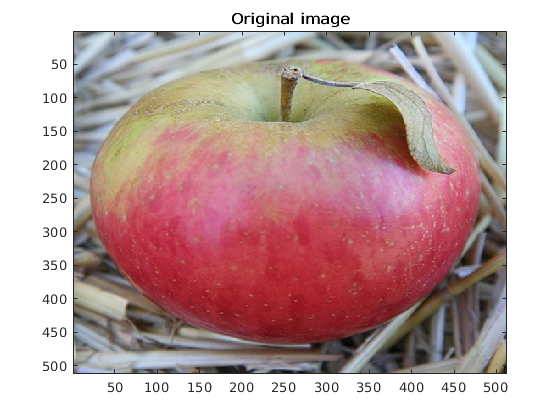
\includegraphics[width=10cm]{apple_orig.png}
  \end{center}
  To train the SVM, $N = 3$ patches of background and $M = 1$ patch of
  the apple were taken as training data. This resulted in the
  following classification:
  \begin{center}
    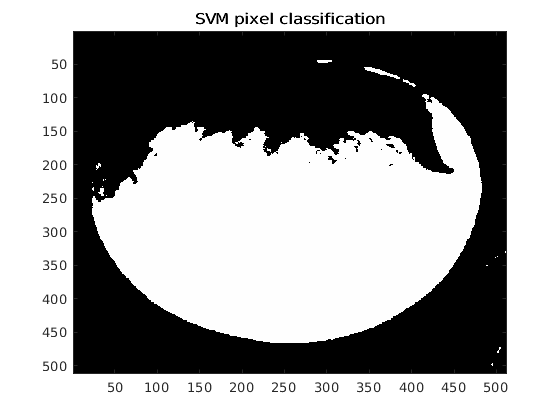
\includegraphics[width=10cm]{apple_svm.png}
  \end{center}
  For comparison, image thresholding yielded
  \begin{center}
    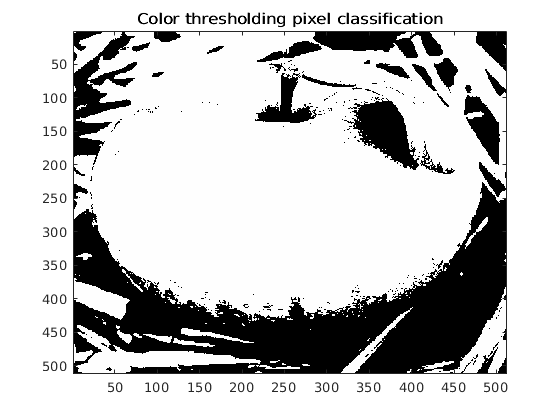
\includegraphics[width=10cm]{apple_color_thresh.png}
  \end{center}
  The SVM picks up most of the apple, particularly parts that are most
  reddish. On the other hand, the color thresholding classifier picks
  up most of the apple, but also incorrectly classifies a great deal
  of the background. The following is the projection of the training
  data onto a 2D subspace perpendicular to the hyperplane computed by
  the SVM:
  \begin{center}
    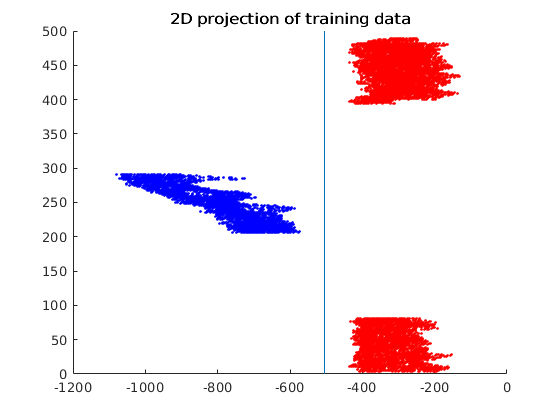
\includegraphics[width=10cm]{apple_proj.png}
  \end{center}
  The red points correspond to the background training observations,
  while the blue points correspond to those taken from the apple. The
  blue line is the projection of the hyperplane. From this projection,
  we see that the SVM classified correctly classified all of the
  training data.

  The original image containing the hand is as follows:
  \begin{center}
    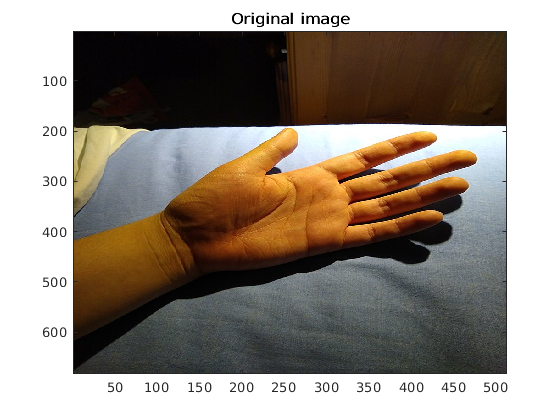
\includegraphics[width=10cm]{hand_orig.png}
  \end{center}
  Classification using the SVM gives the following classification:
  \begin{center}
    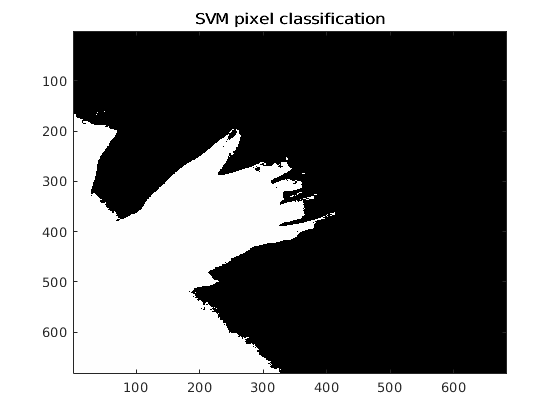
\includegraphics[width=10cm]{hand_svm.png}
  \end{center}
  For comparison, image thresholding yields
  \begin{center}
    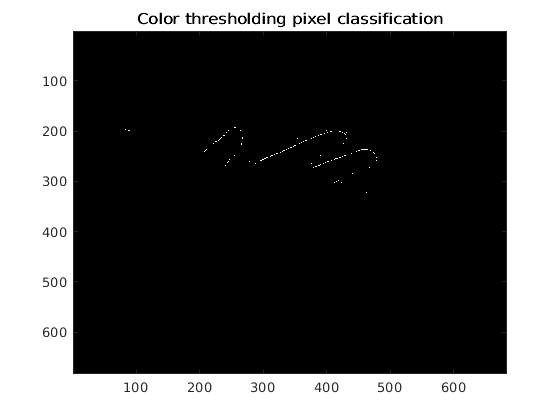
\includegraphics[width=10cm]{hand_color_thresh.png}
  \end{center}
  The SVM picks up most of the hand (excluding the ends of the
  fingers), while color thresholding only picks up part of the outline
  of the fingers. The following is the projection of the training data
  onto a 2D subspace perpendicular to the hyperplane computed by the
  SVM:
  \begin{center}
    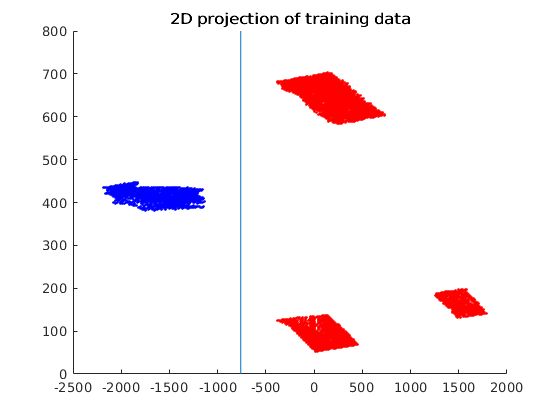
\includegraphics[width=10cm]{hand_proj.png}
  \end{center}
  The red points correspond to the background training observations,
  while the blue points correspond to those taken from the apple. The
  blue line is the projection of the hyperplane. From this projection,
  we see that the SVM classified correctly classified all of the
  training data.

\item (Boyd \& Vandenberghe, Exercise 5.5) The Lagrangian of this
  problem is given by
  \begin{align*}
    L(x, \lambda, \nu)
      &= c^T x + \sum_{i=1}^m \lambda_i (Gx - h)_i
        + \sum_{i=1}^m \nu_i (Ax - b)_i \\
      &= c^T x + \lambda^T (Gx - h) + \nu^T (Ax - b) \\
      &= (c + G^T \lambda + A^T \nu)^T x - \lambda^T h - \nu^T b,
  \end{align*}
  with domain
  $\dom L = \mathbb{R}^n \times \mathbb{R}^m \times \mathbb{R}^p$. The
  Lagrange dual function is therefore
  \begin{equation*}
    g(\lambda, \nu) = \inf_{x \in \mathbb{R}^n} L(x, \lambda, \nu)
      = \inf_{x \in \mathbb{R}^n}
        \left[ (c + G^T \lambda + A^T \nu)^T x - \lambda^T h - \nu^T b \right],
  \end{equation*}
  which is unbounded below unless $c + G^T \lambda + A^T \nu = 0$, in
  which case $g(\lambda, \nu) = -\lambda^T h - \nu^T b$. Therefore,
  \begin{equation*}
    g(\lambda, \nu) = \begin{cases}
      -\lambda^T h - \nu^T b &\quad \text{if $c + G^T \lambda + A^T \nu = 0$} \\
      -\infty &\quad \text{otherwise}.
    \end{cases}
  \end{equation*}
  The dual problem is therefore
  \begin{equation*}
    \begin{array}{ll}
      \text{maximize} & -\lambda^T h - \nu^T b \\
      \text{subject to}
        &\lambda \succeq 0 \\
        &c + G^T \lambda + A^T \nu = 0
    \end{array}.
  \end{equation*}

\item (Boyd \& Vandenberghe, Exercise 5.12) Define a matrix
  $A \in \mathbb{R}^{m \times n}$ by $A = (a_1, \ldots,
  a_m)^T$. Introducing a variable $y \in \mathbb{R}^m$ and
  corresponding equality constraints $y = b - Ax$, the problem can be
  written
  \begin{equation*}
    \begin{array}{ll}
      \text{minimize} & -\sum_{i=1}^m \log y_i \\
      \text{subject to}
        &y = b - Ax
    \end{array}.
  \end{equation*}
  (Note that by definition of the problem domain $\mathcal{D}$, we
  always have $y = b - Ax \succ 0$). The Lagrangian of this problem is
  given by
  \begin{align*}
    L(x, y, \lambda)
      &= -\sum_{i=1}^m \log y_i + \sum_{i=1}^m \nu_i (y + Ax - b)_i \\
      &= -\sum_{i=1}^m \log y_i + \nu^T (y + Ax - b) \\
      &= \left( -\sum_{i=1}^m \log y_i + \nu^T y \right) + \nu^T Ax - \nu^T b,
  \end{align*}
  with domain
  $\dom L = \mathcal{D} \times \mathbb{R}_{++}^m \times
  \mathbb{R}^m$. The Lagrange dual function is therefore
  \begin{align*}
    g(\nu)
      &= \inf_{(x, y) \in \mathcal{D} \times \mathbb{R}_{++}^m} L(x, y, \nu) \\
      &= \inf_{(x, y) \in \mathcal{D} \times \mathbb{R}_{++}^m}
         \left[ \left( -\sum_{i=1}^m \log y_i + \nu^T y \right)
         + \nu^T Ax - \nu^T b \right] \\
      &= \inf_{y \in \mathbb{R}_{++}^m}
         \left( -\sum_{i=1}^m \log y_i + \nu^T y \right)
         + \inf_{x \in \mathcal{D}} (\nu^T Ax) - \nu^T b.
  \end{align*}
  The term $\nu^T Ax$ is unbounded below unless $\nu^TA = 0$ (or
  equivalently, if $A^T \nu = 0$). The term
  $-\sum_{i=1}^m \log y_i + \nu^T y$ is unbounded below unless
  $\nu \succ 0$, in which case the condition
  \begin{equation*}
    \nabla_y \left( -\sum_{i=1}^m \log y_i + \nu^T y \right) = 0
  \end{equation*}
  implies that $y_i = 1 / \nu_i$ for every $1 \leq i \leq m$, and
  since this term is strictly convex in $y$, it attains its unique
  minimum at this point. Therefore,
  \begin{equation*}
    g(\nu) = \begin{cases}
      \sum_{i=1}^m \log \nu_i + m - \nu^T b
        &\quad \text{if $\nu \succ 0$, $A^T \nu = 0$} \\
      -\infty &\quad \text{otherwise}
    \end{cases}.
  \end{equation*}
  The dual problem is therefore
  \begin{equation*}
    \begin{array}{ll}
      \text{minimize} & \sum_{i=1}^m \log \nu_i + m - \nu^T b \\
      \text{subject to}
        &A^T \nu = 0
    \end{array},
  \end{equation*}
  with problem domain
  $\mathcal{E} = \{\nu \in \mathbb{R}^m : \nu \succ 0\}$.

\end{enumerate}

\end{document}
